\documentclass[tikz,border=8pt]{standalone}
\usepackage{fontspec}
\usepackage{xeCJK}
\setmainfont{Times New Roman}
\setCJKmainfont{Hiragino Sans GB}
\setCJKsansfont{Microsoft YaHei}
\setCJKmonofont{STSong}
\usepackage{amsmath}
\usepackage{pgfplots}
\usepackage{xcolor}
\pgfplotsset{compat=1.18}

\definecolor{lineblue}{HTML}{2F6DB2}
\definecolor{linedark}{HTML}{333333}

\begin{document}
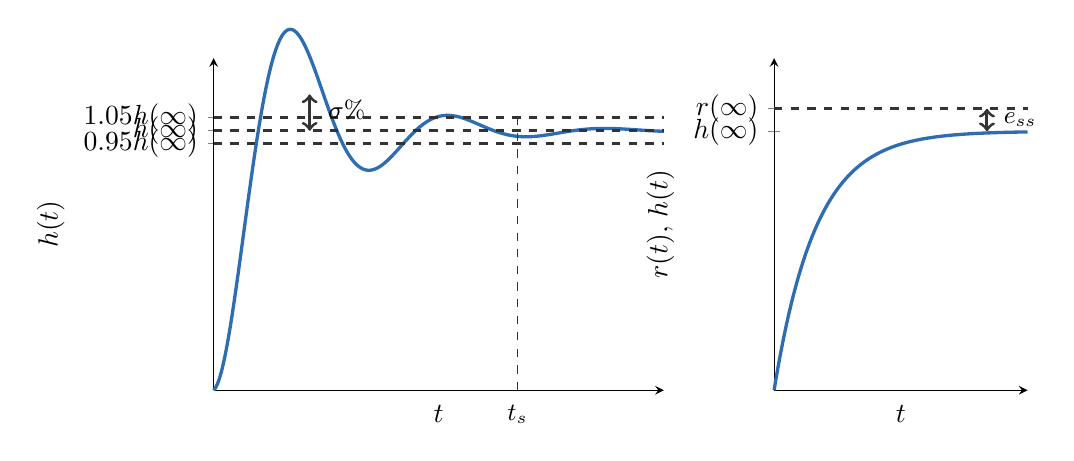
\begin{tikzpicture}
  \begin{axis}[
    name=leftplot,
    width=7.3cm,
    height=5.8cm,
    xmin=0, xmax=6,
    ymin=0, ymax=1.28,
    axis lines=left,
    xlabel={$t$},
    ylabel={$h(t)$},
    xtick=\empty,
    ytick={0.95,1.0,1.05},
    yticklabels={$0.95h(\infty)$,$h(\infty)$,$1.05h(\infty)$},
    every axis plot/.append style={line width=1.2pt, color=lineblue},
    clip=false
  ]
    \addplot[samples=240, domain=0:6] {1 - exp(-0.9*x)*(cos(deg(3*x)) + 0.22*sin(deg(3*x)))};
    \addplot[dashed, color=linedark] coordinates {(0,1.0) (6,1.0)};
    \addplot[dashed, color=linedark] coordinates {(0,1.05) (6,1.05)};
    \addplot[dashed, color=linedark] coordinates {(0,0.95) (6,0.95)};
    \draw[dashed, color=linedark] (axis cs:4.05,0) -- (axis cs:4.05,1.05);
    \node[font=\small, anchor=north] at (axis cs:4.05,-0.02) {$t_s$};
    \draw[<->, line width=1.1pt, color=linedark] (axis cs:1.28,1.0) -- (axis cs:1.28,1.14);
    \node[font=\small, anchor=west] at (axis cs:1.4,1.08) {$\sigma\%$};
  \end{axis}

  \begin{axis}[
    at={(leftplot.east)},
    anchor=west,
    xshift=1.4cm,
    width=4.8cm,
    height=5.8cm,
    xmin=0, xmax=5,
    ymin=0, ymax=1.18,
    axis lines=left,
    xlabel={$t$},
    ylabel={$r(t),\,h(t)$},
    xtick=\empty,
    ytick={0.92,1.0},
    yticklabels={$h(\infty)$,$r(\infty)$},
    every axis plot/.append style={line width=1.2pt},
    clip=false
  ]
    \addplot[color=linedark, dashed, samples=2, domain=0:5] {1};
    \addplot[color=lineblue, samples=180, domain=0:5] {0.92*(1 - exp(-1.2*x))};
    \draw[<->, line width=1.1pt, color=linedark] (axis cs:4.2,0.92) -- (axis cs:4.2,1.0);
    \node[font=\small, anchor=west] at (axis cs:4.34,0.96) {$e_{ss}$};
  \end{axis}
\end{tikzpicture}
\end{document}
